%% SECTION HEADER /////////////////////////////////////////////////////////////////////////////////////
\section{Analytical validation of the \acs{pzt} model}
\label{sec:pztVal}

%% SECTION CONTENT ////////////////////////////////////////////////////////////////////////////////////
The current model, i.e. the curved boundary geometry approximated with the second order elements, is validated by comparing the transducer impedance obtained by numerical simulation and analytical model derived by Giurgiutiu \cite{giurgiutiu2009micromechatronics}.
The impedance Z is a ratio between voltage \((\Phi)\) and current \((I)\) defined as follows:
\begin{eqnarray}
	Z = \frac{\Phi}{I} = \frac{\Phi}{i\omega Q},
\end{eqnarray}
where \(i=\sqrt{-1}\), \(\omega\) is the angular frequency.
In the case of numerical simulation, \(\Phi\) is assumed as the 1.5-cycle Hann windowed sine pulse, and \(Q\) is the charge induced on the electrode calculated by Eq. (\ref{eq:pzt_sem}). 
The excitation signal has significant values in the 0-300 \unit{\kHz} frequency range, as shown in Fig.~\ref{fig:impedance}(\textbf{a}).
The analytical model is defined as:
\begin{eqnarray}
	Z = \frac{1}{i\omega C_0}\left[\left(1-k_p^2\right)+k_p^2\frac{u_r}{u_I}\right],
\end{eqnarray}
where \(C_0\) is the free capacitance of the sensor, \(k_p\) is the planar coupling coefficient, \(u_r\) is the displacement response, and \(u_I\) is the induced displacement.
Additionally, for comparison, the response of the \ac{sem} with curved boundary approximated by linear elements was included. 
\begin{figure}[H]
	\begin{center}
		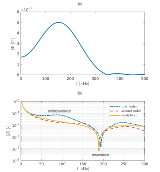
\includegraphics[width=0.95\textwidth]{Chapter_6/impedance}
	\end{center}
	\caption{Validation of the \acf{pzt} model (\textbf{a}) the frequency spectrum of the excitation signal, (\textbf{b}) impedance response of the transducer for analytical model solid line, numerical model with first order approximation of the curved boundary dash-dot line, and numerical model with second order approximation of the curved boundary dashed line.}
	\label{fig:impedance}
\end{figure}

It can be notice in Fig.~\ref{fig:impedance}(\textbf{b}) that the impedance of the model with second order approximation elements is in very good agreement with the analytical solution.
The resonant peak occurred near 190 \unit{\kHz} in both cases, while the resonance of the model with first order approximation elements is shifted 12 \unit{\kHz} toward the higher frequency.
In addition, an antiresonance peak occurred around 90 \unit{\kHz}, which was not observed in the previous two models.